\chapter{tracer\_decay}

\section{Purpose}

To demonstrate that TELEMAC-2D can model the transport of non-conservative
tracer in a flow.

\section{Approach}
The validation is processed with a hypothetical one-dimensional flow with
constant velocity (0.03m/s) and constant depth (10m).

\section{Description}

\subsection{Geometry and mesh}
\begin{itemize}
\item Channel length = 11400m
\item Channel width = 50m
\end{itemize}

Channel Mesh:
\begin{itemize}
\item 2850 triangular elements
\item 1716 nodes
\item Size of triangles = 40m (along the channel bank) *10m (along the channel width)
\end{itemize}

\subsection{Physical parameters}

Initial condition:
\begin{itemize}
  \item The concentration of the tracer is 30mg/l at the left boundary
nodes and 0mg/l at all other nodes.
\item Constant velocity 0.03 m/s
\item Constant water height 10m
\end{itemize}

Boundary conditions:
\begin{itemize}
\item Left inlet boundary:
\begin{itemize}
\item Constant velocity of 0.03m/s
\item Constant tracer concentration of 30 mg/l for first 6 hours, 0 mg/L after.
\end{itemize}
\item Right outlet boundary:
\begin{itemize}
\item Constant velocity of -0.03m/s
\item Free tracer concentration
\end{itemize}
\item Lateral boundaries: solid smooth boundary
\end{itemize}

Bottom:
\begin{itemize}
\item Flat bottom without friction
\end{itemize}

Parameters for non-conservative tracers:
\begin{itemize}
\item Number of tracer: 1
\item Coefficient for diffusion of tracers: 30 m 2 /s
\item Decay rate: 0; 1.0/day; 2.0/day
\end{itemize}

\subsection{Numerical parameters}

Tracer:
\begin{itemize}
\item Advection of tracer: method of characteristics
\item Solver for diffusion of tracer: conjugate gradient method
\item Accuracy: 10 -10
\end{itemize}

Flow and velocity:
\begin{itemize}
  \item No diffusion
  \item No advection
\end{itemize}

Time data:
\begin{itemize}
  \item Time step: 100 sec
  \item Simulation period: 518400 sec (6 days)
\end{itemize}

\section{results}

The tracer concentration time series of analysis and simulation at X =2000m are
compared. Visually the solution produced by TELEMAC-2D shows very good
agreement with the exact solution. For 6 days of simulation duration, when Kd
=0 or Kd=1/day, the model peak time is 5 minutes earlier than the exact peak
time; and for Kd =2, the time difference is less than 2 minutes.

\section{conclusion}
TELEMAC reproduces accurately the transport of non-conservative tracers.

\section{figures}
\begin{figure}
\centering
  \includegraphicsmaybe{[width=.6\textwidth]}{../img/mesh.png}
\caption{Full mesh}\label{fig:tracer_decay:mesh}
\end{figure}

\begin{figure}
\centering
  \includegraphicsmaybe{[width=.6\textwidth]}{../img/mesh_zoomed.png}
\caption{Zoomed mesh}\label{fig:tracer_decay:mesh_zoomed}
\end{figure}

\begin{figure}
\centering
  \includegraphicsmaybe{[width=.6\textwidth]}{../img/tracer_t0.png}
\caption{Initial state of tracer}\label{fig:tracer_decay:tracer_t0}
\end{figure}

\begin{figure}
\centering
  \includegraphicsmaybe{[width=.6\textwidth]}{../img/tracer_t0_zoomed.png}
\caption{Initial state of tracer zoomed}\label{fig:tracer_decay:tracer_t0_zoomed}
\end{figure}

\begin{figure}
\centering
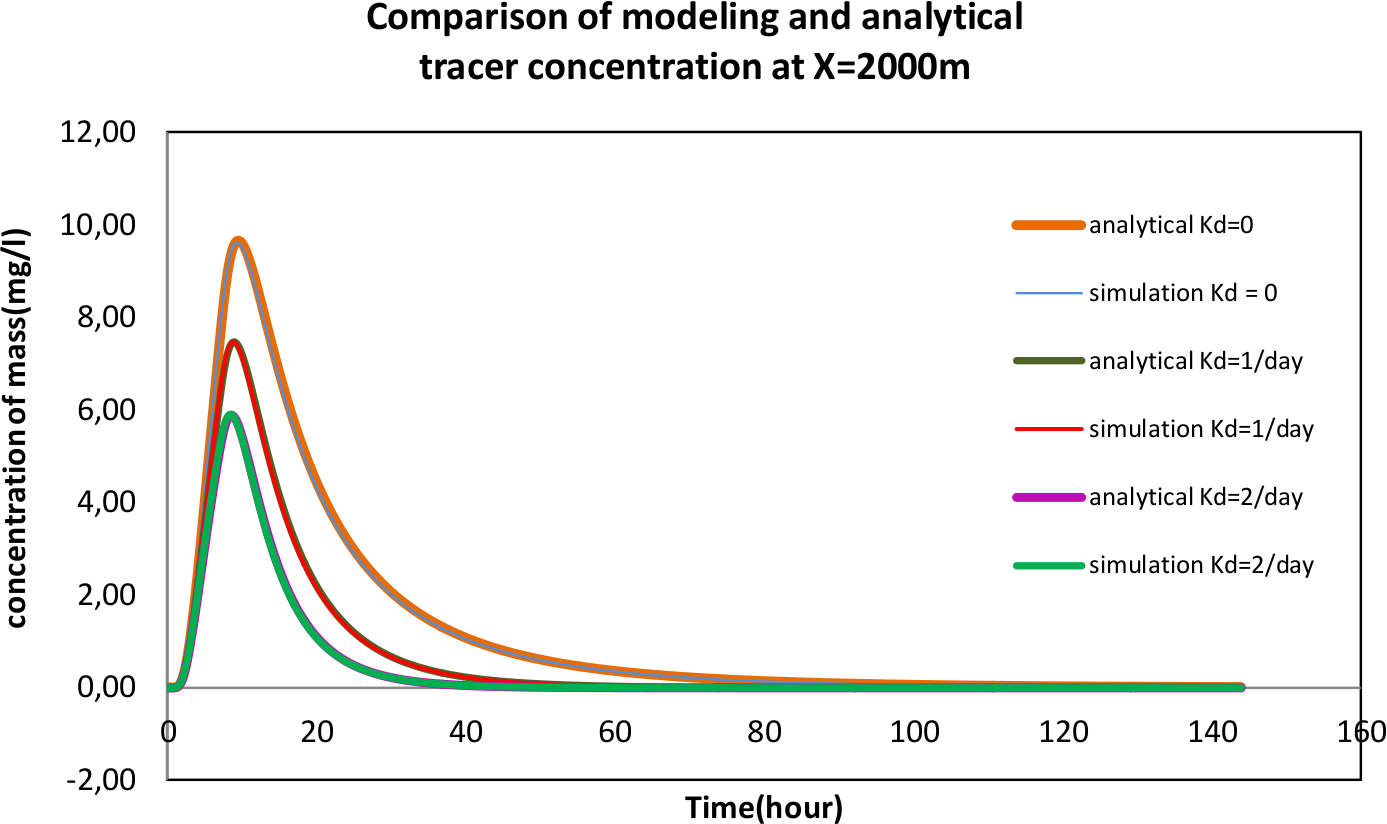
\includegraphics[width=.6\textwidth]{img/sol_anal}
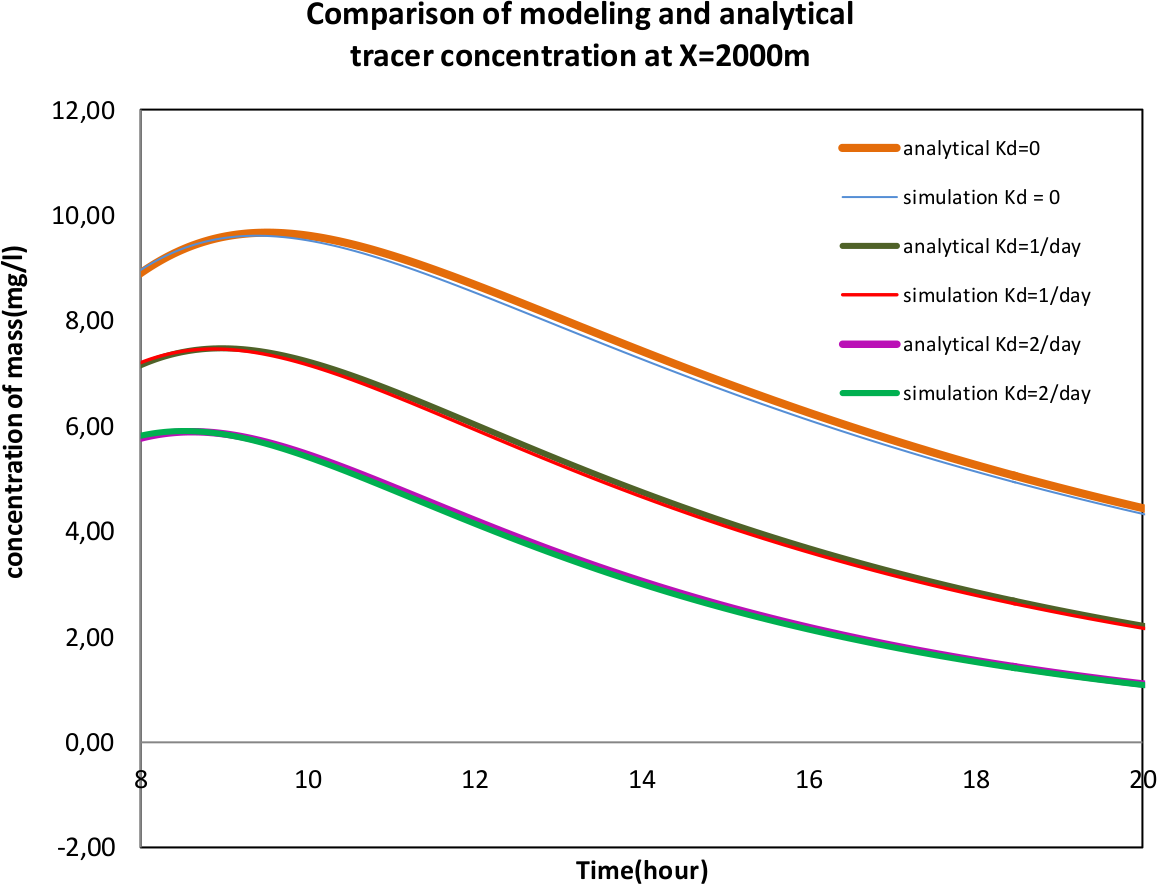
\includegraphics[width=.6\textwidth]{img/sol_anal_zoomed}
\caption{Comparison between analytical solution and telemac-2D solution for non-conservative tracer transport}\label{fig:tracer_decay:sol_anal}
\end{figure}
